\documentclass[11pt]{article}
\usepackage{graphicx}

\begin{document}
\title{Homework 14}
\author{Colt Bradley}
\date{}
\maketitle

\section{Part 1}

We evaluate the integral of $\sin$ from $0$ to $\pi /2$ using the midpoint method for various steps. When we graph the Log error of the integral against the Log steps the graph is linear. 

\begin{figure}[ht]
\centering
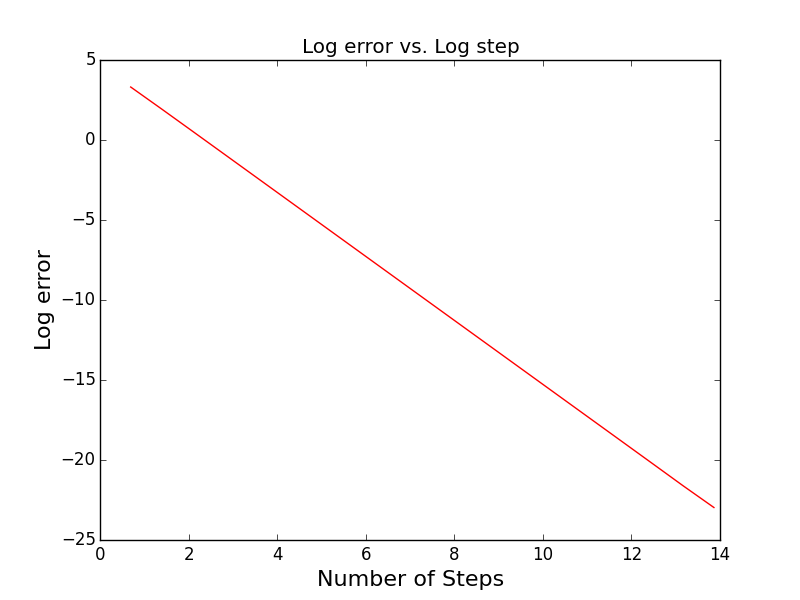
\includegraphics[scale=.5]{logerror.png}
\end{figure}

\section{Part 2}

\subsection{Integral 1}

This first integral is infinite at zero, so we encounter some issues when we use the midpoint method to evaluate. When the number of steps is even, we don't evaluate at zero and get a small error. When the number of steps is odd, we evaluate at zero and the calculation blows up. 

\begin{equation}
I_1 = \int_{-1}^{1} \frac{1}{x^{2/3}}
\end{equation}

\subsection{Integral 2}

The second integral is also infinite at zero, but we encounter different issues. When the number of steps is odd, the integral is infinite. When the number of steps is even the integral is a lot less. 

\begin{equation}
I_2 = \int_{-1}^{1} \frac{1}{x^{2}}
\end{equation}

\section{Code}

\begin{verbatim}
#Colt Bradley
#3.3.16
#Lesson 14

import numpy as n
import pylab as p


#########################################################################
#Exercise 1
#########################################################################

a = 0
b = n.pi/2
N = 20
h = (b-a)/N
I_m = 0
i = 1
I = []
err = []

r = n.zeros(N)
r[0] = 2
for i in range(0,N-1):
    r[i+1] = 2*r[i]

def f(x):
    k = n.sin(x)
    return k

#middle
for k in r:
    I = []
    i = 0
    I_m = 0
    h = (b-a)/k
    while i < k+1:
        I_m = I_m + f(a+i*h-h/2)*h
        i = i+1
        I.append(I_m)
    err.append(abs(1-I[-1])*100)

err = n.log(err)
r = n.log(r)

p.close()
p.title("Log error vs. Log step")
p.plot(r,err,"r")
p.ylabel("Log error",fontsize = 16)
p.xlabel("Number of Steps",fontsize = 16)
p.show()

#########################################################################
#Exercise 2
#########################################################################


a = -1
b = 1.
N = 5
h = (b-a)/N
I_m = 0
i = 1
I = []

def f(x):
    k = 1./((x)**(2./3))
    return k


while i < N+1:
    I_m = I_m + f(abs(a+i*h-h/2))*h
    i = i+1
    I.append(I_m)
print(abs((6-I_m)))

#########################################################################
#Exercise 3
#########################################################################

a = -1
b = 1.
N = 41
h = (b-a)/N
I_m = 0
i = 1
I = []

def f(x):
    k = 1./((x)**(2.))
    return k


while i < N+1:
    I_m = I_m + f(abs(a+i*h-h/2))*h
    i = i+1
    I.append(I_m)
print(abs((6-I_m)))

\end{verbatim}




\end{document}